\documentclass[a4paper,12pt]{article} % тип документа

% Поля страниц
\usepackage[left=2.5cm,right=2.5cm, top=2cm,bottom=2cm,bindingoffset=0cm]{geometry}

%Пакет дял таблиц   
\usepackage{multirow} 

%Отступ после заголовка    
\usepackage{indentfirst}


% Рисунки
\usepackage{subcaption,floatrow,graphicx,calc}
\usepackage{wrapfig}

% Создаёем новый разделитель
\DeclareFloatSeparators{mysep}{\hspace{1cm}}

% Ссылки?
\usepackage{hyperref}
\usepackage[rgb]{xcolor}
\hypersetup{				% Гиперссылки
	colorlinks=true,       	% false: ссылки в рамках
	urlcolor=blue          % на URL
}


%  Русский язык
\usepackage[T2A]{fontenc}			% кодировка
\usepackage[utf8]{inputenc}			% кодировка исходного текста
\usepackage[english,russian]{babel}	% локализация и переносы


% Математика
\usepackage{amsmath,amsfonts,amssymb,amsthm,mathtools, mathrsfs, wasysym}


\begin{document}
	\begin{center}
		\footnotesize{ФЕДЕРАЛЬНОЕ ГОСУДАРСТВЕННОЕ АВТОНОМНОЕ ОБРАЗОВАТЕЛЬНОЕ 			УЧРЕЖДЕНИЕ ВЫСШЕГО ОБРАЗОВАНИЯ}\\
		\footnotesize{МОСКОВСКИЙ ФИЗИКО-ТЕХНИЧЕСКИЙ ИНСТИТУТ\\(НАЦИОНАЛЬНЫЙ 			ИССЛЕДОВАТЕЛЬСКИЙ УНИВЕРСИТЕТ)}\\
		\footnotesize{ФАКУЛЬТЕТ ОБЩЕЙ И ПРИКЛАДНОЙ ФИЗИКИ\\}
		\hfill \break
		\hfill\break
		\hfill\break
		\hfill \break
		\hfill \break
		\hfill \break
		\hfill \break
		\hfill \break
		\hfill \break
		\hfill \break
		\hfill \break
		\hfill \break
		\hfill \break
		\hfill \break
		\large{Лабораторная работа № 6.11.5 \\\textbf{Туннелирование в полупроводниках.}}\\
		\hfill \break
		\hfill \break
		\hfill \break
		\begin{flushright}
			Серебренников Даниил\\
			Группа Б02-826м
		\end{flushright}
		\hfill \break
		\hfill \break
		\hfill \break
		\hfill \break
		\hfill \break
		\hfill \break
		\hfill \break
		\hfill \break
		\hfill \break
		\hfill \break
		\hfill \break
	\end{center}
	\begin{center}
		Долгопрудный, 2021 г.
	\end{center}
	\thispagestyle{empty}
	\newpage
	\textbf{Цель работы:} исследовать принцип действия туннельного диода, измерить его ВАХ и основные параметры.
	
	\section{Основные формулы}
	Расстояния от уровня Ферми до краев зон:
	\begin{equation*}
		\begin{gathered}
			\xi = \mu_n - E_c,\\
			\eta = \mu_p - E_v.
		\end{gathered}
	\end{equation*}

	 При достижении $U_v$ ток через диод минимален, что соответсвуетсвует совпадению границ зоны проводимости $E_c$ и валентной зоны $E_v$. Откуда можно оценить положение уровней Ферми:
	\begin{equation*}
		eU_v \approx \xi + \eta \approx 2\xi \approx 2\eta.
	\end{equation*}

	Напряжению $U_p$ соответствует пик тока, при котором смещение энергетических зон должно быть одинаково. Это даёт возможность определить энергетический промежуток $E_{n \max}$ между уровнем Ферми и максимум плотности распределения электронов $n_{\max}(E)$, отсчитываемый от границы зоны проводимости:
	\begin{equation*}
		eU_p \approx \xi - E_{n\max}.
	\end{equation*}



	\section{Экспериментальная установка}
	Для измерения основных параметров туннельного диода используется монтажная плата, на которой собраны три схемы для снятия ВАХ, схема для наблюдения ВАХ на экране осцил-лографа и схема генератора электро-магнитных колебаний в туннельном диоде.
	\begin{equation*}
		I_\text{д} = U_Y = \frac{R_1 + 2(R_2 + R_3)}{(R_1 + 2R_2)R_3}.
	\end{equation*}
	
	
	\newpage
	\section{Экспериментальные данные}
	Масштаб по осям X и Y: 2В/дел.
	\begin{figure}[h!]
		\begin{floatrow}
			\ffigbox[\FBwidth]{\caption{ВАХ туннельного диода.}\label{fig:osc1}}%
			{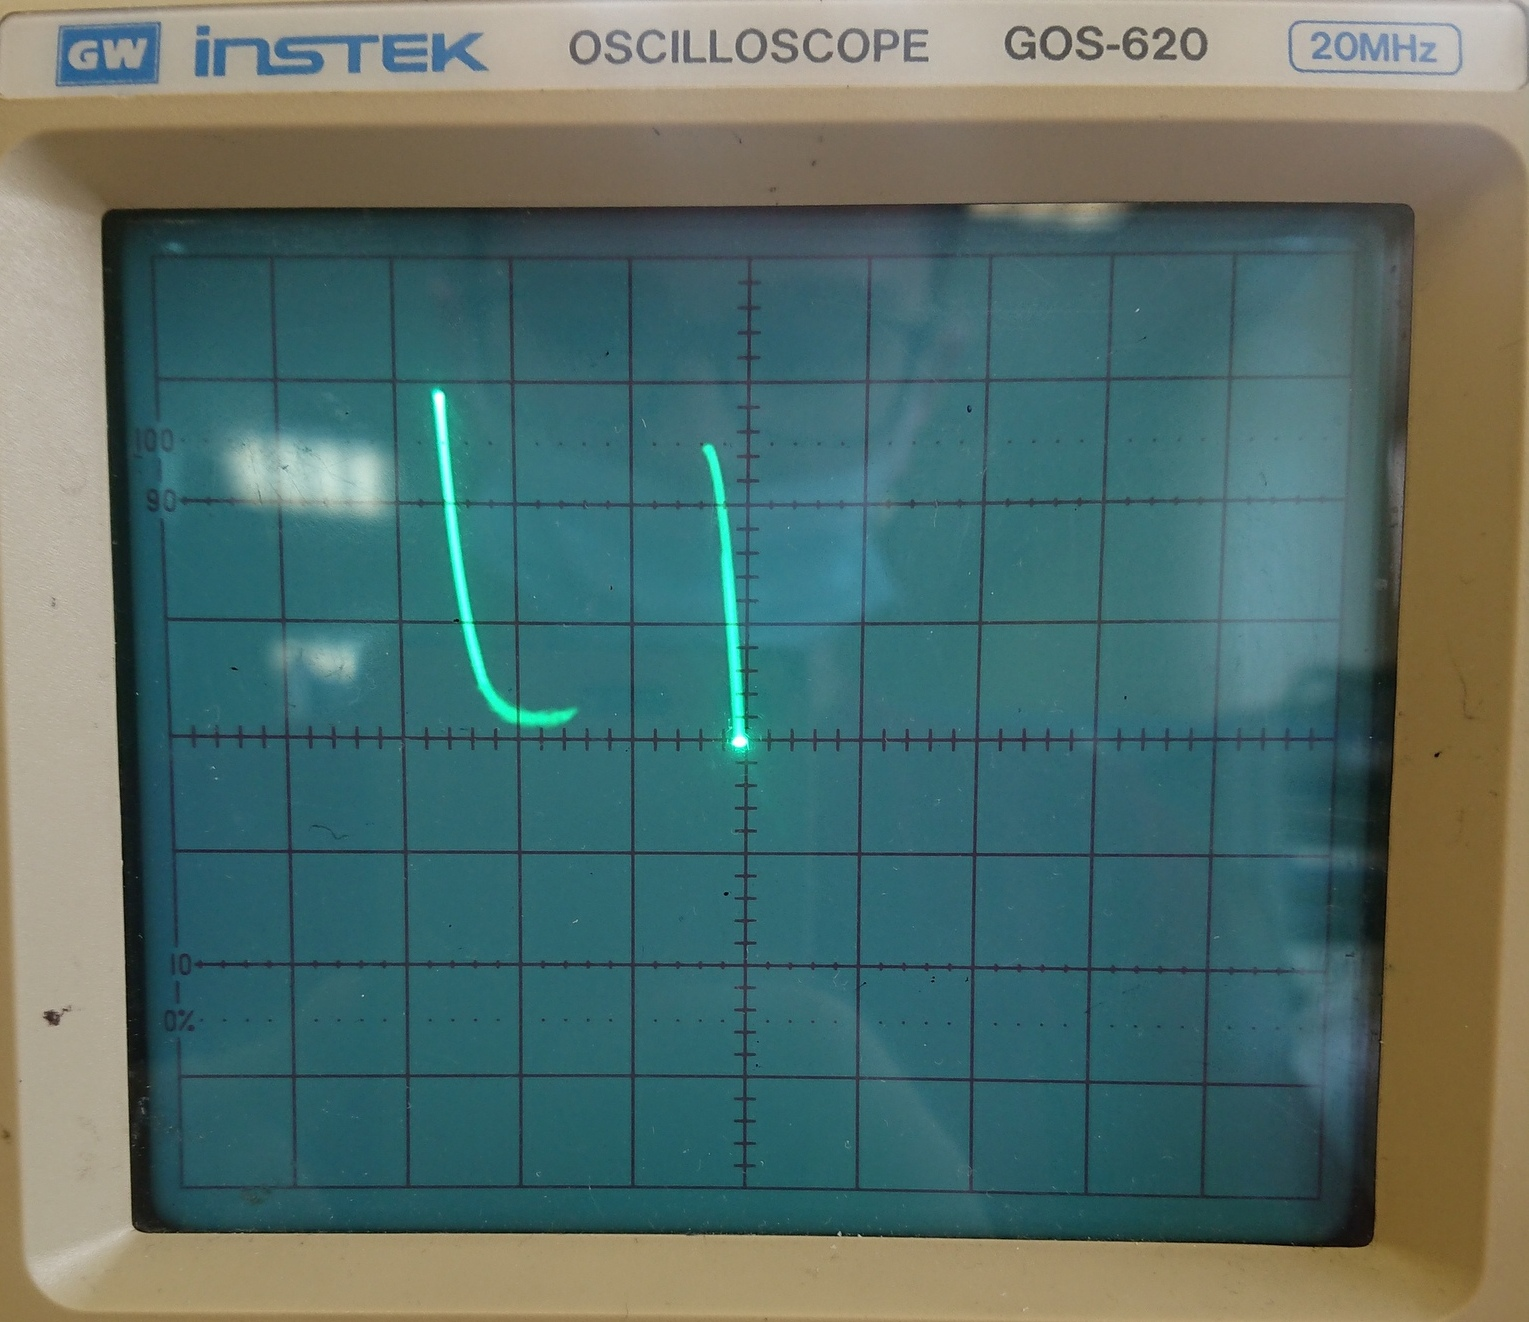
\includegraphics[scale=0.18]{osc1}}
			\ffigbox[\FBwidth]{\caption{ВАХ диода.}\label{fig:osc2}}%
			{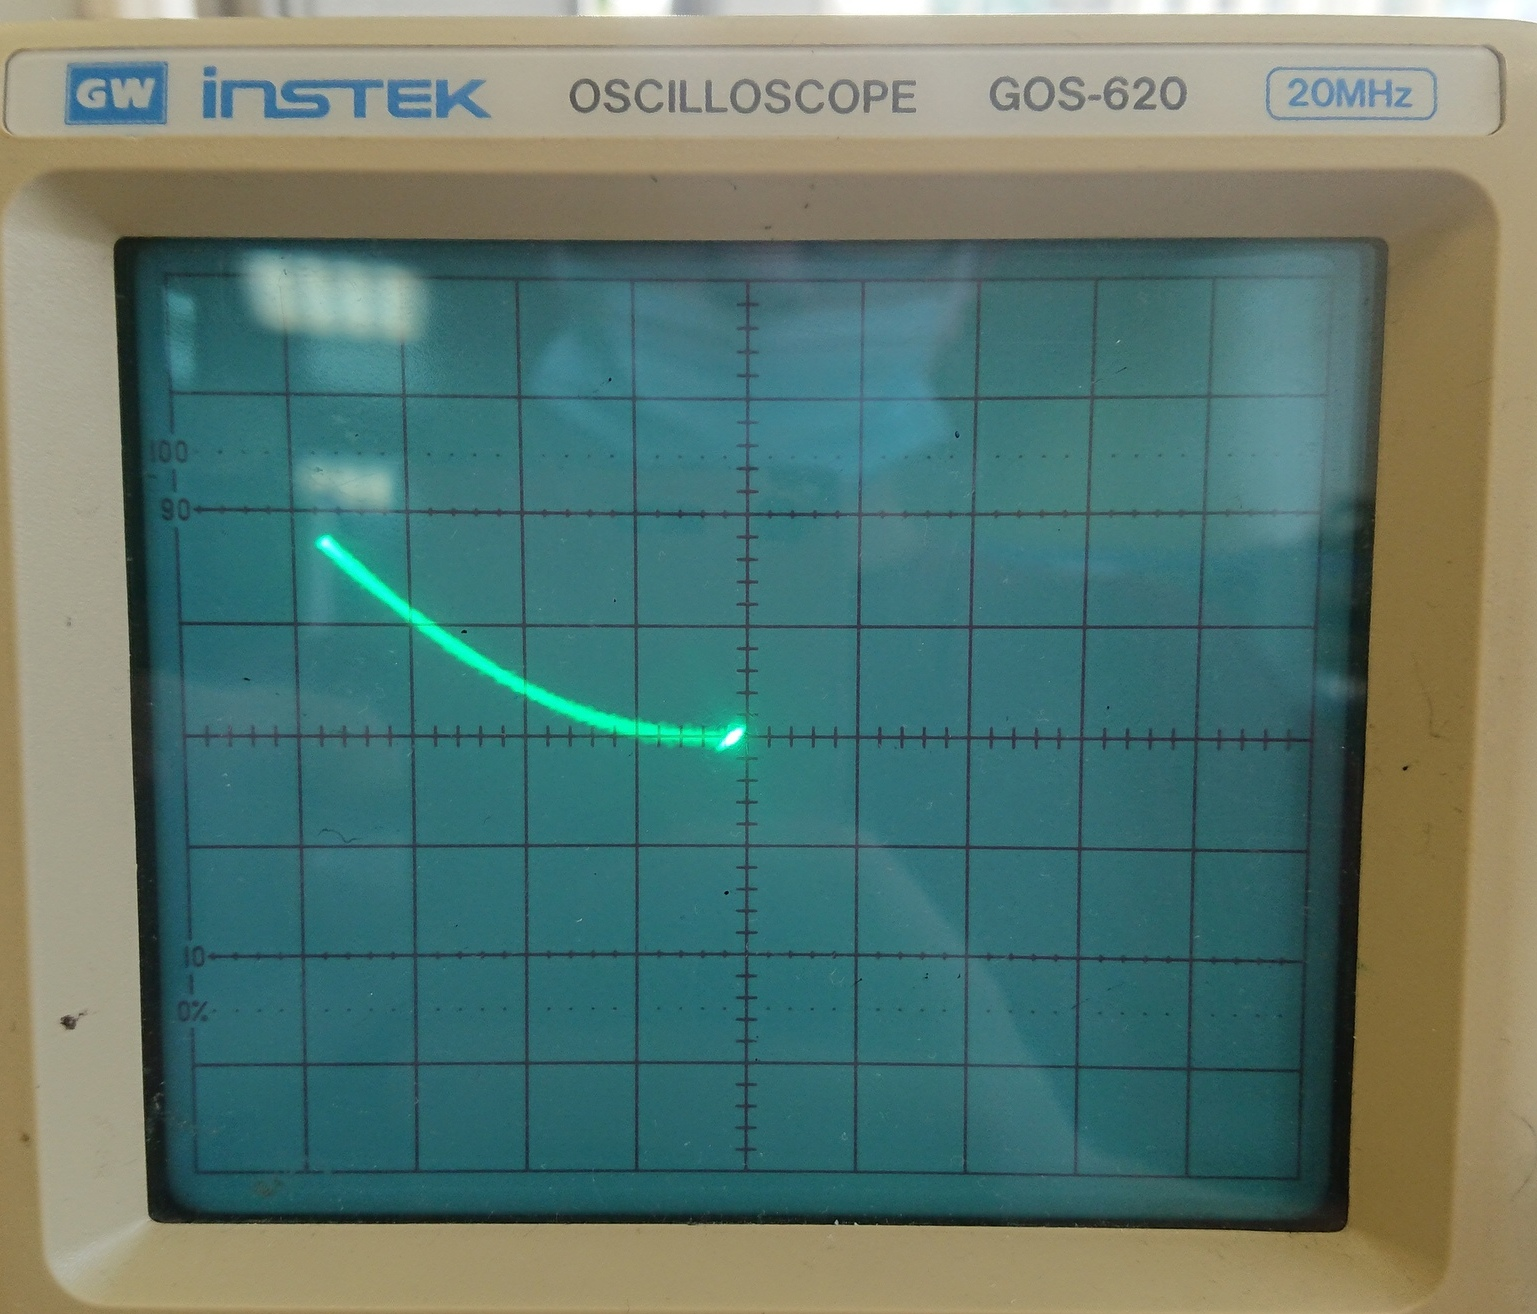
\includegraphics[scale=0.18]{osc2}}     
		\end{floatrow}
	\end{figure}
	
	\floatsetup[table]{capposition=top}	
	\begin{table}[H]
		\caption{Результаты измерений.}
		\label{table:exp1}
		\begin{tabular}{|c|c|c|c|}
			\hline
			\multicolumn{2}{|c|}{Туннельный диод} & \multicolumn{2}{c|}{Обычный диод} \\ \hline
			$V$, мВ           & $I$, мА           & $V$, мВ         & $I$, мА         \\ \hline
			10,0              & 1,72              & 1,5             & -0,021          \\ \hline
			20,5              & 3,04              & 64,7            & -0,004          \\ \hline
			32,4              & 4,03              & 76              & 0,11            \\ \hline
			350               & 0,85              & 121             & 0,06            \\ \hline
			373               & 0,74              & 181             & 0,16            \\ \hline
			400               & 0,63              & 210             & 0,24            \\ \hline
			432               & 0,99              & 239             & 0,32            \\ \hline
			447               & 1,33              & 280             & 0,47            \\ \hline
			464               & 1,93              & 292             & 0,52            \\ \hline
			488               & 3,78              & 325             & 0,66            \\ \hline
			493               & 4,47              & 355             & 0,8             \\ \hline
			2,30              & 0,40              & 389             & 0,98            \\ \hline
			3,00              & 0,53              & 406             & 1,07            \\ \hline
			4,00              & 0,70              & 468             & 1,46            \\ \hline
			5,30              & 0,93              & 473             & 1,49            \\ \hline
			8,00              & 1,38              & 584             & 2,31            \\ \hline
			265               & 1,50              & 609             & 2,52            \\ \hline
			37,0              & 4,13              & 622             & 2,62            \\ \hline
			32,8              & 4,05              &                 &                 \\ \hline
			224               & 2,07              &                 &                 \\ \hline
			330               & 1,04              &                 &                 \\ \hline
			250               & 1,72              &                 &                 \\ \hline
			378               & 0,71              &                 &                 \\ \hline
		\end{tabular}
	\end{table}
	Погрешность измерений: $\pm$ единица к последнему разряду.
	
	
	\newpage
	\section{Обработка результатов}
	\thisfloatsetup{floatrowsep=mysep}	
	\begin{figure}[h!]
		\begin{floatrow}
			\ffigbox[\FBwidth]{\caption{Зависимость концентрации от энергии.}\label{fig:f(x)}}
			{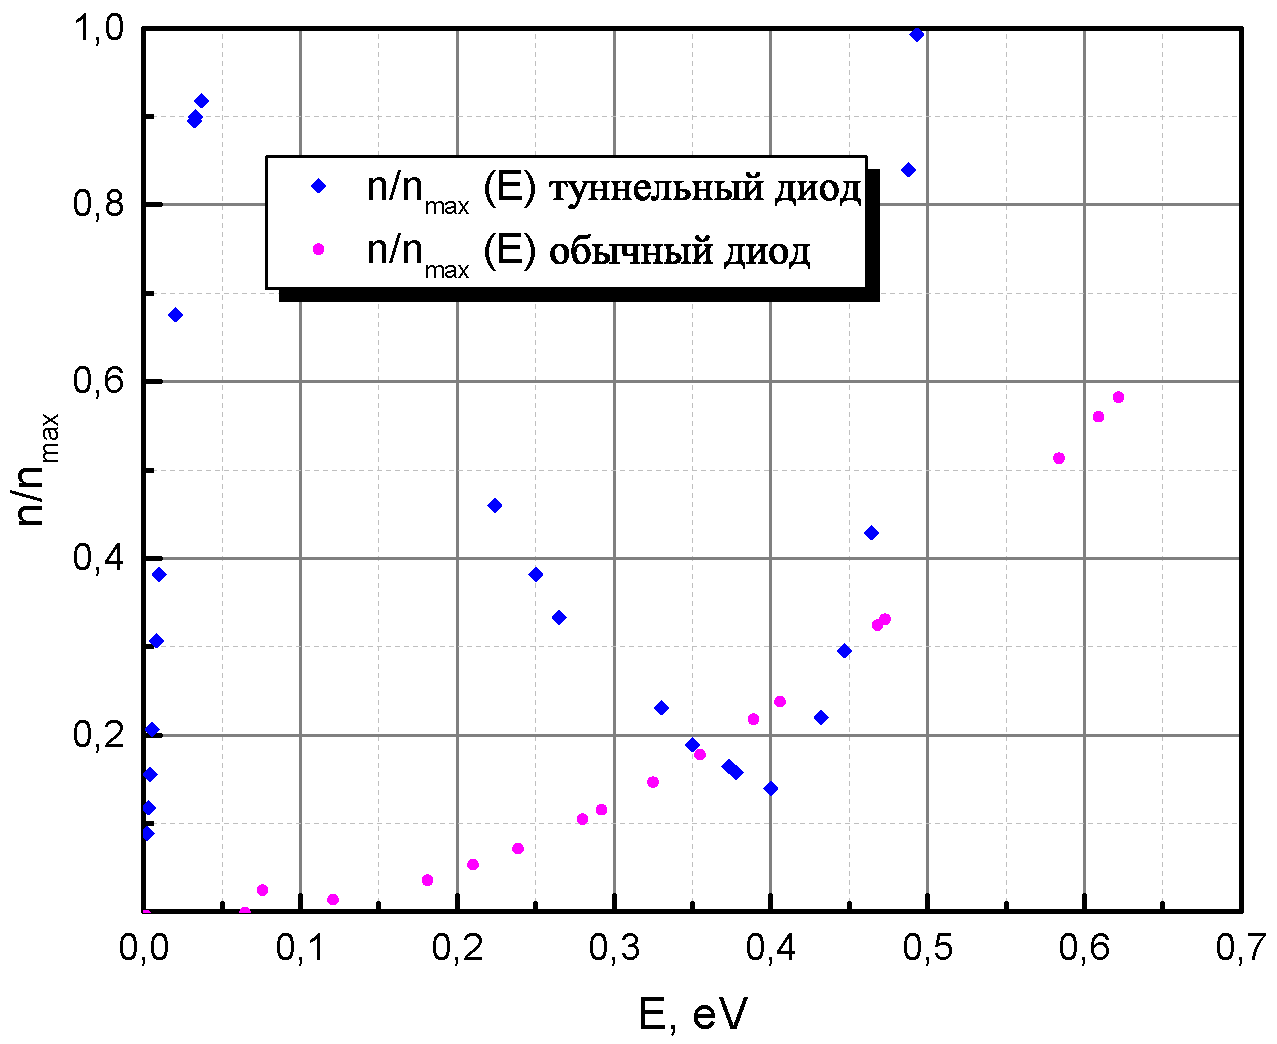
\includegraphics[scale=0.5]{graph.pdf}}    
		\end{floatrow}
	\end{figure}
	$$eU_p = (0,05 \pm 0,01)\text{эВ}, \ eU_v = (0,40 \pm 0,01)\text{эВ}, \ eU_f = (0,50 \pm 0,01) \text{эВ} . $$

	\[\boxed{\xi = eU_v/2 = (0,20 \pm 0,01) \text{эВ} }\]
	\[\boxed{E_{n \max} = \xi - eU_p = (0,15 \pm 0,02) \text{эВ}}\]
	
	Параметры генератора: $0,1\,\text{МГц}\le f \le 0,2\,\text{МГц} $, $97\, \text{мВ} \le A \le 242\, \text{мВ}$.
	
	\section{Обсуждение результатов и выводы}
	В ходе лабораторной работе была получена статическая вольт-амперная характеристика туннельного диода и на осциллографе. Оценили положение уровня Ферми и максимума распределения электронов в зоне проводимости полупроводника туннельного диода.
	
\end{document}